\documentclass[11pt, a4paper]{article}


%%%% Encodings

\usepackage[utf8]{inputenc} % encoding
\usepackage[english]{babel} % use special characters and also translates some elements within the document.

%%%% Misc

\usepackage{hyperref}       % Hyperlinks \url{url} or \href{url}{name}
\usepackage{parskip}        % \par starts on left (not idented)
\usepackage{tocbibind}      % Adds the bibliography to the table of contents (automatically)

% \usepackage[document]{ragged2e}  % Left-aligned (whole document)
% \begin{...} ... \end{...}   flushleft, flushright, center

%%%% Abstract

\usepackage{abstract}       % Abstract

% http://www.ctex.org/documents/packages/special/abstract.pdf
\renewcommand{\absnamepos}{flushleft} % \begin{abstract} \noindent ... \end{abstract}
\setlength{\absleftindent}{0pt}
\setlength{\absrightindent}{0pt}

%%%% Graphics

\usepackage{graphicx}
\graphicspath{ {./figs/} } % directory to look up for graphics

% \begin{figure}[h]
%   \centering
%   \includegraphics[scale=0.5]{cat}  % [width=\textwidth, height=4cm],
%   \caption{Example of a cat}
%   \label{fig:cat}
% \end{figure}

%%%% Math

\usepackage{amsmath}        % Math
\usepackage{amssymb}        % New symbols http://milde.users.sourceforge.net/LUCR/Math/mathpackages/amssymb-symbols.pdf
\usepackage{bm}             % $\bm{D + C}$

\usepackage{amsthm} % Math, \newtheorem, \proof, etc
% \begin{theorem}\label{t:label}  ...  \end{theorem}
% \begin{proof} ... \end{proof}
\theoremstyle{plain} % default
\newtheorem{theorem}{Theorem}[section]
\newtheorem{corollary}{Corollary}[theorem]  % Numering depends on the current section (instead of global)
\newtheorem{lemma}[theorem]{Lemma} % Shares numeration with theorem.
\theoremstyle{definition}
\newtheorem{definition}{Definition}[section]
\theoremstyle{remark}
\newtheorem*{remark}{Remark}

% Defines a new environment to write your or claim - proof
\newenvironment{claim}[1]{\par\noindent\underline{Claim:}\space#1}{}
\newenvironment{claimproof}[1]{\par\noindent\underline{Proof:}\space#1}{\hfill $\blacksquare$}

%%%% Code/Pseudo-code

\usepackage{minted} % Code listing
% \mint{html}|<h2>Something <b>here</b></h2>|
% \inputminted{octave}{BitXorMatrix.m}

%\begin{listing}[H]
  %\begin{minted}[xleftmargin=20pt,linenos,bgcolor=codegray]{haskell}
  %\end{minted}
  %\caption{Example of a listing.}
  %\label{lst:example} % You can reference it by \ref{lst:example}
%\end{listing}

\newcommand{\code}[1]{\texttt{#1}} % Define \code{foo.hs} environment

\usepackage[vlined,ruled]{algorithm2e} % pseudo-code http://tug.ctan.org/macros/latex/contrib/algorithm2e/doc/algorithm2e.pdf

%%%% Colors

\usepackage{xcolor}         % Colours \definecolor, \color{codegray}
\definecolor{codegray}{rgb}{0.9, 0.9, 0.9}
% \color{codegray} ... ...
% \textcolor{red}{easily}

%%%% Math

%\makeglossaries % before entries

%\newglossaryentry{latex}{
    %name=latex,
    %description={Is a mark up language specially suited
    %for scientific documents}
%}

% Referene to a glossary \gls{latex}
% Print glossaries \printglossaries

\usepackage[acronym]{glossaries} %

% \acrshort{name}
% \acrfull{name}
% \newacronym{foo}{arcshort}{acrfull}

\usepackage{enumitem} % \begin{enumerate}[label=(\alph*)]



\renewcommand{\thesection}{\Alph{section}}
\renewcommand{\thesubsection}{\thesection.\arabic{subsection}}

\usepackage{fancyhdr}
\usepackage{listings}
\usepackage{graphicx}
\pagestyle{fancy}
\fancyhf{}
\rhead{OD}
\lhead{FIB - UPC}
\rfoot{Page \thepage}

\title{%
  \vspace{-10ex}
  OD: Lab Assignment 1
}
\author{%
  Antoni Casas \\
  Arnau Abella \\
  \\
  \large{Universitat Polit\`ecnica de Catalunya}
}
\date{\today}

%%%%%%%%%%%%%%%%%%%%%%%%%%%%%%%%%%%%%%%%%%%%%%%%%%%%%%%%%

\begin{document}
\maketitle

%%%%%%%%%%%%%%%% Section A
\section{Modeling, Loading, Evolving}%

%%%%%% Subsection A.1
\subsection{Modeling}%
\label{sub:modeling}

\label{sec:modeling_loading_evolving}
\begin{figure}[H]
  \center
  \makebox[\textwidth][c]{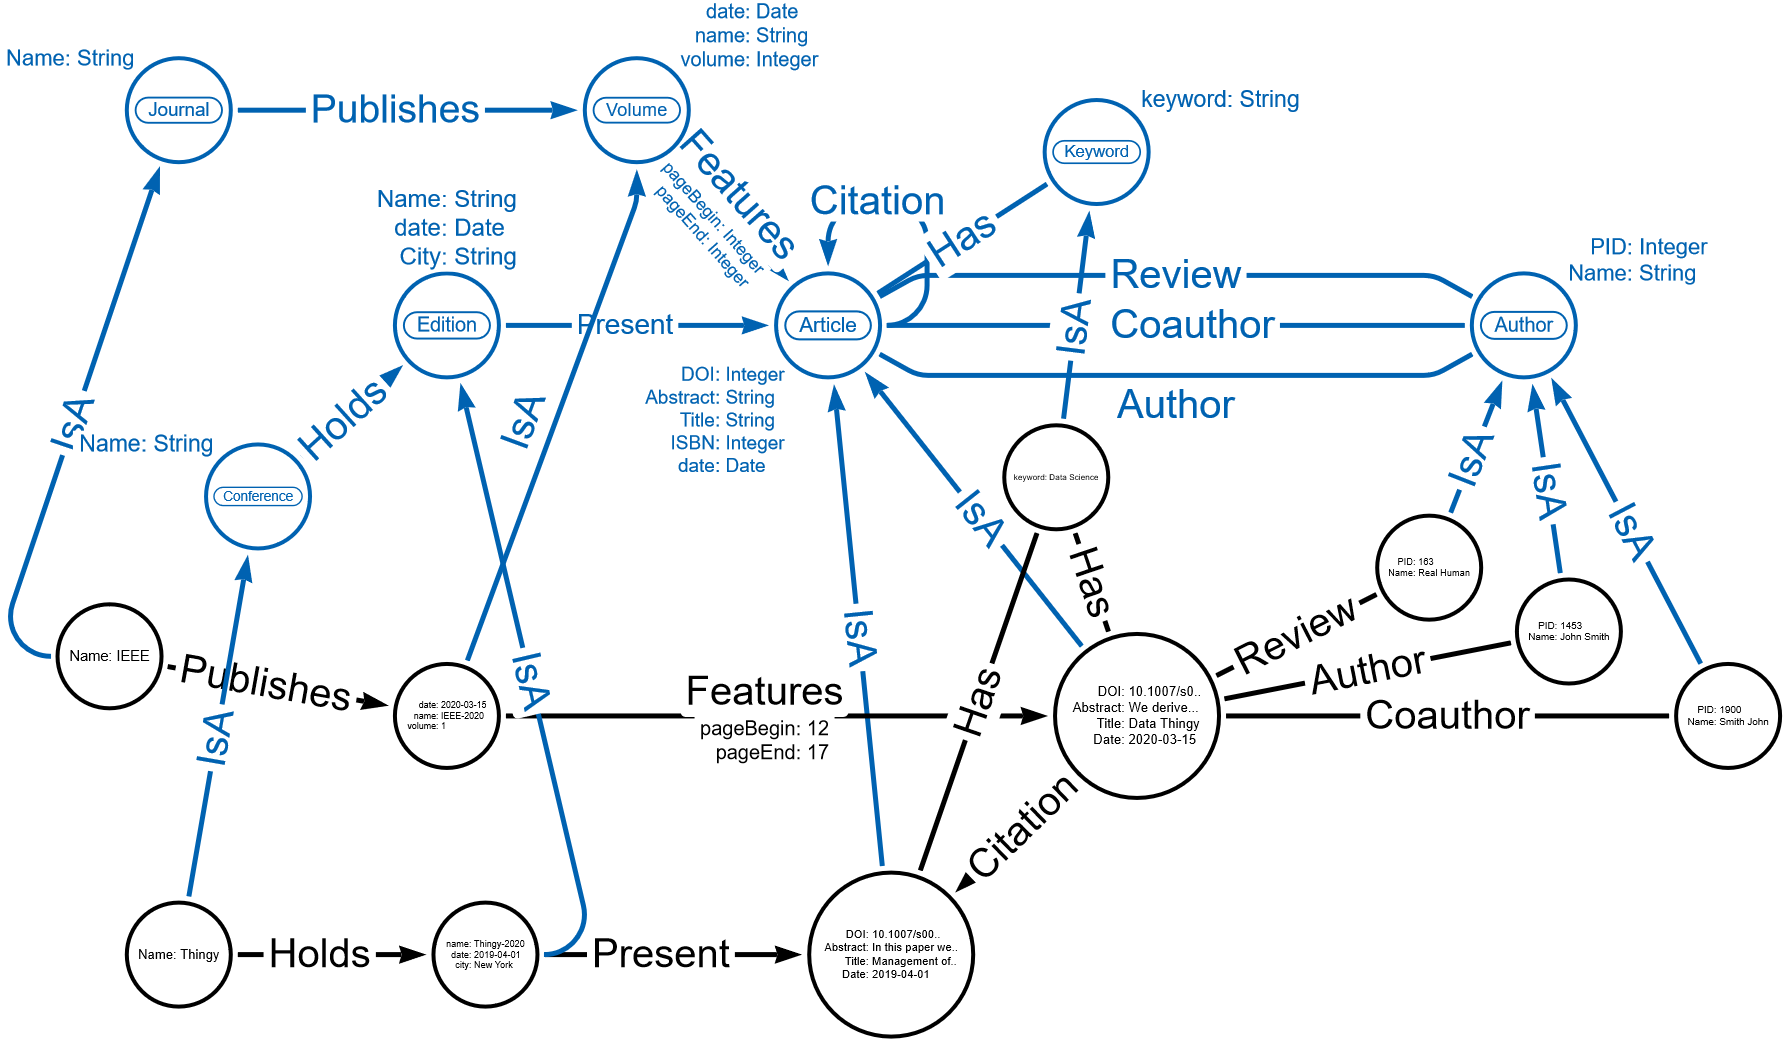
\includegraphics[width=1.3\textwidth]{Graph.png}}
  \caption{Data Model}
  \label{fig:modifiedGraph}
\end{figure}

Conferences and Journals are kept different due to their semantic differences, even if they could be the same node, data wise.

Conferences can hold events freely, and journals can publish volumes freely, however these must hold articles.

Articles are compromised of their doi, abstract, title and publish date, this date can be used to express differences such as an article being published somewhere before being presented in the edition of the conference, or being published in somewhere like ArxiV before being published in a journal, but also it allows further efficiency when having to obtain the article's date for the impact factor query.

Every author is also a coauthor, author only expresses that such an author is the primary author of that article.

%%%%%% Subsection A.2
\subsection{Instantiating/Loading}%
\label{sub:instantiating_loading}

In order to instantiate the data for the model of subsection \ref{sub:modeling} there is a quite involved process with the following steps:

\begin{enumerate}
  \item Extract the DOIs of the articles from the DBLP CSV's (see \code{doiExtraction.py}).
  \item Retrieve from \textit{Semantic Scholar} all the information related to the articles (see \code{retrieveAll.py}).
  \item Pre-process the retrieved data and transform it to the corresponding CSVs that are going to be involved in the loading process (see \code{recordsToCSV.py}).
  \item Load the data into \textit{Neo4j} (see \code{loadNeo4j.py}).
\end{enumerate}

The script \code{recordsToCSV.py} does some additional transformation the data from Semantic Scholar since, in some queries, it was not given the expected results:

\begin{itemize}
  \item Conferences and Journals are synthetically created in order to create a suitable topology for the queries.
  \item Editions and Volumes too.
  \item Reviewers are randomly selected among all the authors excluding themselves.
  \item Keywords are artifically added to make the queries in D possible
\end{itemize}

All the original and synthetic data can be found at \code{partA2/data}.
%%%%%% Subsection A.3
\subsection{Evolving the graph}%
\label{sub:evolving_the_graph}

\begin{figure}[H]
  \center
  \makebox[\textwidth][c]{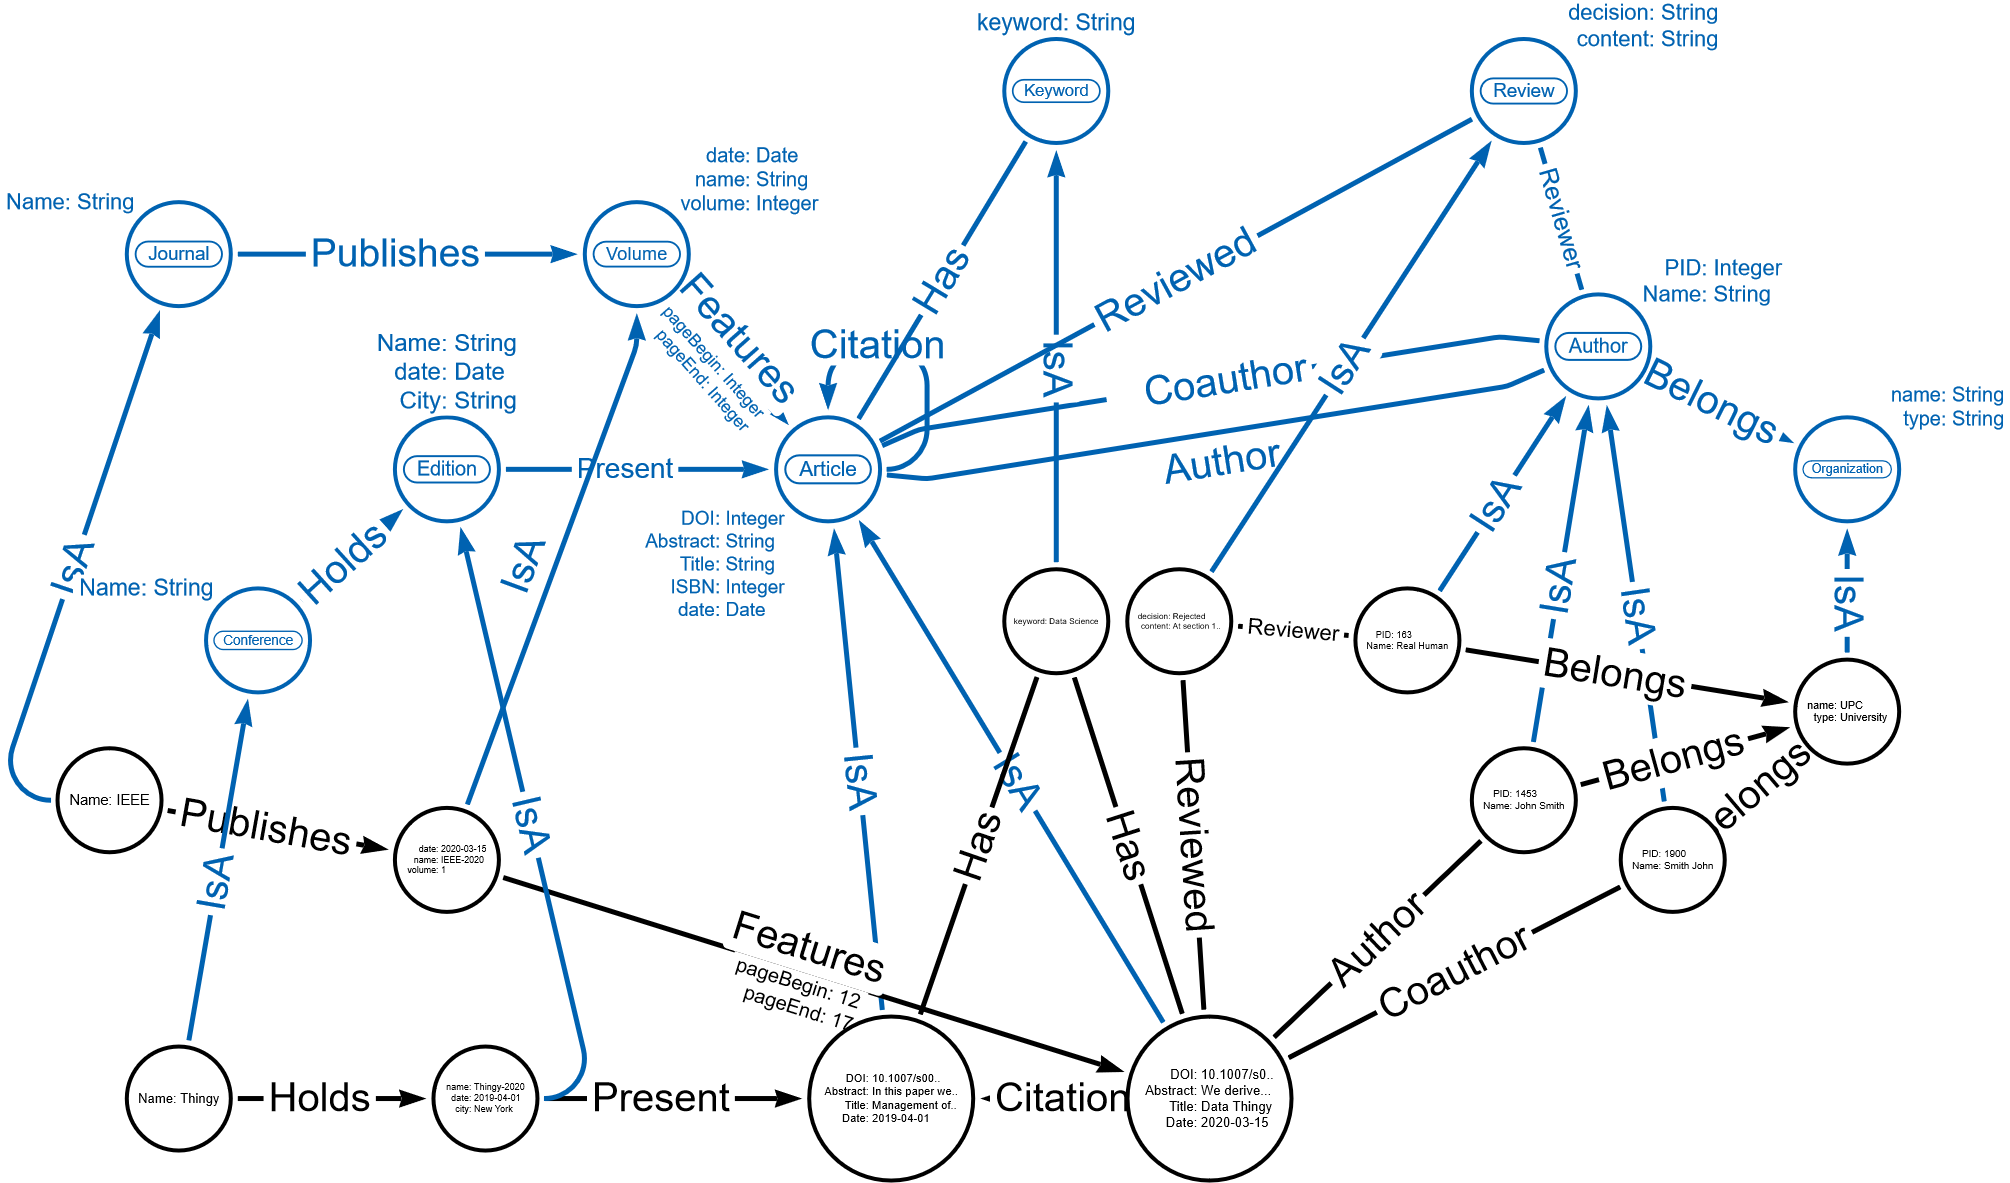
\includegraphics[width=1.3\textwidth]{Graph2.png}}
  \caption{Modified Graph}
  \label{fig:modifiedGraph}
\end{figure}


To adapt the graph to contain the new information, we make the following 2 changes. First, we remove the old relationship of Reviewer we had from author to article, and replace it with a relation to a node Review, which holds the review's contents and its acceptance status, and this node is related to the author who made this review and the article which it reviews.

Secondly, we add a new node, Organization, which stores the organizations, and this node is related to authors, representing via this relationship the organization the author belongs to.

%%%%%%%%%%%%%%%% Section B
\section{Querying}%
\label{sec:querying}

\subsection{Query 1}
\begin{lstlisting}[
    basicstyle=\tiny
]
MATCH ((conf:Conference)-[:Holds]-(edi:Edition)-[:Present]-(art:Article)-[cit:Citation]->(art2:Article))
WITH conf,art,count(cit) as citations ORDER BY conf, count(cit) DESC
WITH conf, collect([art,citations]) AS toCut UNWIND toCut[0..3] AS cut RETURN conf,cut[0],cut[1];
  \end{lstlisting}

This query finds the top 3 most cited papers of each conference. To do this, it first obtains the path match obtaining every citation a conference has had, then it aggregates this on unique conferences and articles, obtaining the count of citations of each article. Then, it aggregates these in order to return only the first 3 per conference.

\subsection{Query 2}
\begin{lstlisting}[
    basicstyle=\tiny
]
MATCH ((conf:Conference)-[:Holds]-(ed:Edition)-[:Present]-(Art:Article)-[:Coauthor]-(aut:Author))
WITH conf,aut,count(DISTINCT ed) as numEds
WHERE numEds>3
RETURN conf,aut;
  \end{lstlisting}

This query finds for each conference find its community: those authors that have published paperson that conference in, at least, 4 different editions. To do this, it first obtains the patch match obtaining for each conference and edition held, all the coauthors, then it aggregates by conference and author, to count the number of different editions, selecting over those aggregations where the number of editions is over 3.

\subsection{Query 3}
\begin{lstlisting}[
    basicstyle=\tiny
]
MATCH ((jor:Journal)-[pub:Publishes]-(vol:Volume)-[:Features]-(art:Article))
WHERE vol.date.year>($year-3) AND vol.date.year>$year
OPTIONAL MATCH ((art:Article)-[cit:Citation]->(cited:Article))
WHERE cited.date.year=$year
WITH count(cited) AS cited, count(art) as publications, jor
RETURN (cited*1.0) / (publications*1.0) AS IF,jor,$year AS year
 \end{lstlisting}

This query finds  the  impact  factor  of  the  journals for \$year. To do this, it first obtains all the articles published the 2 years before \$year by each journal, then, it optionally matches those articles with their citations, and selects those citations in \$year. Obtaining this way the total count of articles in the previous 2 years, and the citations of the year.

\subsection{Query 4}
\begin{lstlisting}[
    basicstyle=\tiny
]
MATCH ((aut:Author)-[:Coauthor]-(art:Article))
OPTIONAL MATCH ((art:Article)-[cit:Citation]->(art2:Article))
WITH aut, art, count(cit) as citation
ORDER BY aut, citation DESC
WITH aut,COLLECT(citation) AS citations
RETURN aut,citations
\end{lstlisting}

This query finds  the  h-indexes  of  the  authors. To do this, it first obtains the path belonging, for each main author, to their published articles, then optionally matching it with the citations, this to also obtain authors that haven't been cited (h-index of 0), then it aggregates by author and article, obtaining the amount of citations per article, then it collects these in order, to be processed outside of Neo4J in a simple for loop.

%%%%%%%%%%%%%%%% Section C
\section{Graph algorithms}%
\label{sec:graph_algorithms}

\subsection{Page Rank}%
\label{sub:page_rank}

%The first selected algorithm is the \textit{Page Rank} \cite{Page98thepagerank}. The algorithm returns the relevance of each node in the network. The revelance of a node is computed by the sum of the relevance of the adjance nodes. The Page Rank is an iterative algorithm. The equation to compute the page rank ($PR$) of a node is the following

%\begin{equation}
  %PR(n_i)  = \frac{1-d}{N} + d \sum_{n_j \in adj(n_i)} \frac{PR(n_j)}{E(n_j)}
%\end{equation}

%\quad where $0 \leq d \leq 1$ is the \textit{damping factor}, $N$ is the total number of nodes in the graph, $adj(n_i)$ are the adjacent nodes of node $i$, $E(n_j)$ is the total number of edges of node $j$.

Page Rank is used in our graph to measure the relevance of an article. The traditional approach of estimating the relevance by the number of references can be considered na\"ive since it does not take into account the relevance of the references. For example, an article with 20 relevant citations should be more relevant that another article with 25 non-relevant citations.

For running page rank on our graph we prepared a \textit{python} script (see \code{partC/pageRank.py}) which prints the page rank of each node in descending order.

\begin{lstlisting}[basicstyle=\tiny,breaklines=false]
CALL gds.pageRank.stream($graphName)
YIELD nodeId, score
RETURN gds.util.asNode(nodeId).title AS name, score
ORDER BY score DESC, name ASC
LIMIT $limit
\end{lstlisting}

Table \ref{table:pagerank} includes the most relevant articles with respect to its page rank in our database.

\begin{centering}
\begin{table}[H]
\makebox[\textwidth]{%
  \begin{tabular}{c|c}
  Title & Page Rank \\ \hline
    \textit{Quad trees a data structure for retrieval [\ldots]}  & $155.4$ \\
  \textit{A fast algorithm for Steiner trees}  & $80.4$ \\
  \textit{The log-structured merge-tree (LSM-tree)}  & $62.8$ \\
  \textit{Concurrency of operations on B-trees}  & $58.3$ \\
  \textit{The temporal logic of branching time}  & $58.2$ \\
  \textit{Amounts of nondeterminism in finite automata}  & $46.1$ \\
  \textit{Subtyping for session types in the pi calculus}  & $31.1$ \\
    \textit{The SB-tree an index-sequential structure [\ldots]}  & $30.4$ \\
  \textit{Optimal scheduling for two-processor systems}  & $26.2$ \\
  \textit{Branching processes of Petri nets}  & $23.9$ \\
  \end{tabular}
}
\caption{Top 10 most relevant papers w.r.t. Page Rank}
\label{table:pagerank}
\end{table}
\end{centering}

\subsection{Louvain Method}%
\label{sub:louvain_method}

%The second selected algorithm is the \textit{Louvain method} \cite{Blondel_2008} for community detection in large networks. The algorithm finds communities by optimizing the \textit{modularity} of the graph. The modularity is defined as

%\begin{equation}
  %Q = \frac{1}{2m}\sum_{ij}\Big[ A_{ij} - \frac{k_i k_j}{2m} \Big] \delta(c_i, c_j)
%\end{equation}

%where

%\begin{itemize}
  %\item $m$ is the sum of all the edge weights of the graph.
  %\item $A_{ij}$ is the edge weight between nodes $i$ and $j$.
  %\item $k_{i}, k_{j}$ are the sum of weights of the edges attached to nodes $i$ and $j$, respectively.
  %\item $c_i, c_j$ are the communities of the nodes.
  %\item $\delta$ is the \textit{Kronecker delta function} ($\delta(x, y) = 1 \text{ if } x = y, 0 \text{ otherwise}$).
%\end{itemize}

%\begin{figure}[H]
  %\center
  %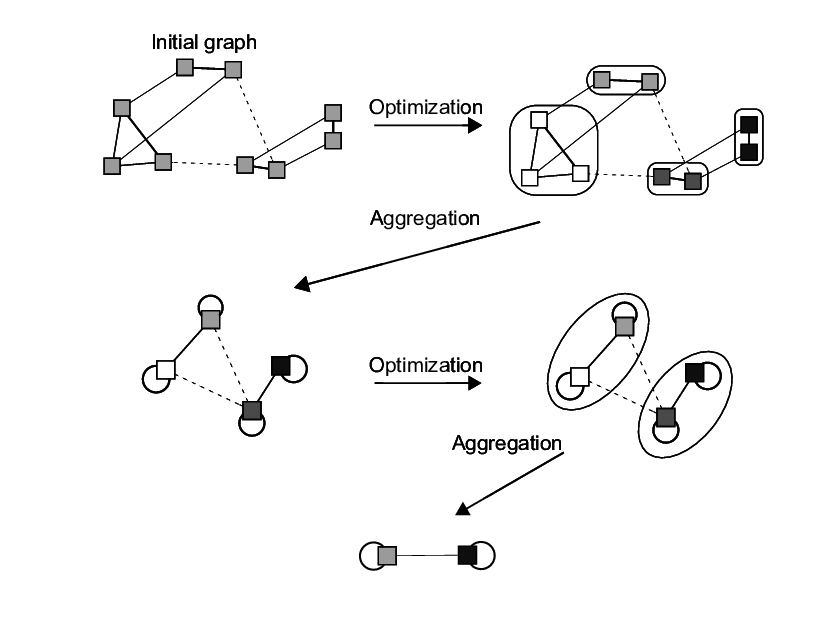
\includegraphics[width=.4\textwidth]{louvain.png}
  %\caption{Louvain method}
  %\label{fig:louvain}
%\end{figure}

%The Louvain method is a two phases iterative algorithm. In the first phase (optimization), the algorithm compute the increment of modularity of moving node $i$ to the neighboring communities $j$, the best movement is picked. This process is repeatedly applied to each node until modularity is maximized. The second phase (aggregation) consist of merging nodes from the same community.

The Louvain method can be applied to our graph, in particular to the articles nodes, to find related articles. We prepared a script (see \code{partC/louvain.py}) to run the Louvain method and find the hidden communities. The following script is part of the code to obtain the communities from our graph.

\begin{lstlisting}[basicstyle=\tiny,breaklines=false]
CALL gds.louvain.stream($graphName)
YIELD nodeId, communityId
RETURN gds.util.asNode(nodeId).title AS title, communityId
ORDER BY communityId ASC
\end{lstlisting}

In table \ref{table:louvain} we display the largests communities in our graph which contains 449 communities in total. For each community we will display its size and three randomly selected articles that belong to the community. Although our database does not contain the topic of the articles, it is clear that the communities are related by topic of publication. For example, community 2 is about tree data structures, community 5 is about program verification, community 6 is about programming language theory, and so on.

\begin{table}[H]
\footnotesize
\makebox[\textwidth]{%
  \begin{tabular}{|c|c|l|}
    \hline
    Community & Size & Articles \\ \hline
    $1$ & $86$ &
    \begin{tabular}[l]{@{}l@{}}
        \textit{M-nets: An algebra of high-level Petri nets  [\ldots]}\\
        \textit{On Gurevich's theorem on sequential algorithms}\\
        \textit{Branching processes of Petri nets}\\
    \end{tabular}\\ \hline
    $2$ & $73$ &
    \begin{tabular}[l]{@{}l@{}}
        \textit{A fast algorithm for Steiner trees} \\
        \textit{Applications of efficient mergeable heaps for optimization problems on trees}\\
        \textit{On efficient implementation of an approximation algorithm for the Steiner tree problem}\\
    \end{tabular}\\ \hline
    $3$ & $71$ &
    \begin{tabular}[l]{@{}l@{}}
        \textit{Quad trees a data structure for retrieval on composite keys}\\
        \textit{Picture deformation}\\
        \textit{Dynamic multi-dimensional data structures based on quad and k-d trees} \\
    \end{tabular}\\ \hline
    $4$ & $70$ &
    \begin{tabular}[l]{@{}l@{}}
        \textit{An algorithmic and complexity analysis of interpolation search}\\
        \textit{Optimal merging of 2 elements with n elements}\\
        \textit{A characterization of database graphs admitting a simple locking protocol}\\
    \end{tabular}\\ \hline
    $5$ & $67$ &
    \begin{tabular}[l]{@{}l@{}}
        \textit{The ‘Hoare logic’ of concurrent programs}\\
        \textit{General predicate transformer and the semantics [\ldots]}\\
        \textit{Specification and verification of database dynamics}\\
    \end{tabular}\\ \hline
    $6$ & $51$ &
    \begin{tabular}[l]{@{}l@{}}
        \textit{The clean termination of iterative programs}\\
        \textit{Duality in specification languages: a lattice-theoretical approach}\\
        \textit{The clean termination of Pascal programs}\\
    \end{tabular}\\
  \hline
  \end{tabular}
}
\caption{Communities found by Louvain method.}
\label{table:louvain}
\end{table}
%%%%%%%%%%%%%%%% Section D

\section{Recommender}%
\label{sec:recommender}

\subsection{Query 1}

\begin{lstlisting}[basicstyle=\tiny]
MERGE (comm: Community{name: $name})
WITH comm
MATCH (kw: Keyword)
WHERE kw.keyword in $keywords
MERGE (comm)-[:Related]-(kw)
\end{lstlisting}

This query creates a community (if it does not exist) and the relationships between the community and the keywords that define it.

\subsection{Query 2}

\begin{lstlisting}[basicstyle=\tiny,breaklines=false]
MATCH (n)-[:Holds|Publishes]-()-[:Present|Features]-(art:Article)
OPTIONAL MATCH (art:Article)-[:Has]-(kw: Keyword)
WITH n, count(distinct art) as total, sum(CASE WHEN kw.keyword in $keywords THEN 1 ELSE 0 END) as subtotal
WHERE subtotal/total >= 0.9
MATCH (comm: Community{name: $name})
MERGE (n)-[:Belongs]-(comm)
RETURN n.name as name
\end{lstlisting}

This query finds conferences and journals related to each community and creates the relationship between them.

\subsection{Query 3}
\begin{lstlisting}[basicstyle=\tiny,breaklines=false]
%Obtain Cypher projection

CALL gds.graph.drop('commCalc')

CALL gds.graph.create.cypher('commCalc',
MATCH (c:Community {name: '\$community'})-[:Belongs]-()-[]-()-[]-(art:Article) RETURN id(art) as id,
MATCH ((c:Community {name: '"+communityName+"'})-[:Belongs]-()-[]-()-[]-(art:Article))
MATCH (art)-[:Citation]->(art2:Article)-[]-()-[]-()-[:Belongs]-(c)
RETURN id(art) as source, id(art2) as target)
YIELD graphName, nodeCount, relationshipCount, createMillis

%Obtain pagerank from projection

CALL gds.pageRank.stream('commCalc')
YIELD nodeId, score RETURN gds.util.asNode(nodeId).doi AS doi,score ORDER BY score DESC LIMIT 100;

%Generate top100 relation

MATCH (art:Article) WHERE art.doi IN $doiList
MATCH (comm:Community {name: $commName})
MERGE (art)-[:Top100]-(comm)
\end{lstlisting}

The first part of query 3 obtains, for a single \$community its projection made of only articles that belong to it, with the relation of their citations, it is done this way due to RAM limitations when performing page rank due to its high demand for RAM, performing page rank with the projection of only one community at a time.

The second part of the query performs the page rank, and finally, the third part, uses the list of doi obtained to generate a relation from each of the articles belonging to it to its community, the Top100 relation. All this is repeated for each community

\subsection{Query 4}
\begin{lstlisting}[basicstyle=\tiny,breaklines=false]
MATCH (aut:Author)-[:Coauthor]-(art:Article)-[:Top100]-(c:Community)
WITH aut,c,count(art) AS articles
MERGE (aut)-[:ReviewCandidate]-(c)
WITH aut,c,articles
WHERE articles>1
MERGE (aut)-[:ReviewGuru]-(c)
\end{lstlisting}

Query 4 uses the relation obtained in query 3, the Top100, to obtain all authors belonging to it, then creates the ReviewCandidate relation with their corresponding community, then, if the author has more than 1 article, then it also creates the ReviewGuru relation.
%%%%%%%%%%%%%%%%%%%%%%%%%%%%%%%%%%%%%%%%%%%%%%%%%%%%%%%%%

%\bibliographystyle{unsrt}
%\bibliography{refs}

\end{document}
